\documentclass[]{article}
\usepackage{amsmath}
\usepackage{amsthm}
\usepackage{amssymb}
\usepackage{graphicx}
\usepackage[utf8]{inputenc} 
\usepackage{subcaption}
\usepackage{caption}
\usepackage{hyperref}
\usepackage{amsbsy}
\usepackage[left=4cm]{geometry}
 %http://tex.stackexchange.com/questions/595/how-can-i-get-bold-math-symbols
%opening
\title{Variance reduction in coarse bifurcation analysis of stochastic models}
\author{Pieter Van Nuffel}

\newcommand{\R}{\ensuremath{\mathbb{R}}} % commando zonder argumenten
\newcommand{\C}{\ensuremath{\mathbb{C}}}
\newcommand{\N}{\ensuremath{\mathbb{N}}}
\newcommand{\E}{\ensuremath{\mathbb{E}}}
\newcommand{\norm}[1]{\left\|#1\right\|} % commando's met argumenten
\newcommand{\pa}[2]{\frac{\partial #1}{\partial #2}}
\newcommand{\ppa}[2]{\frac{\partial^2 #1}{\partial #2^2}}
\newcommand{\dd}{\ensuremath{\mathrm{d}}}
\newcommand{\U}{\ensuremath{\boldsymbol{\rho}}}
\newcommand{\cts}{\ensuremath{\boldsymbol{\Phi}^N_T}} %Coarse time step
\newcommand{\V}{\ensuremath{\mathbf{v}}} 
\newcommand{\jv}{\ensuremath{\mathbf{\hat{Jv}}}}
\newcommand{\jvpde}{\ensuremath{\mathbf{Jv}_{FP}}}

\theoremstyle{definition}
\newtheorem{Theorem}{Theorem}


\begin{document}



 
\section{Model problem}



\subsection{Advection-diffusion}

In general, we are interested in performing a bifurcation analysis for  models at which an exact, closed model at the macroscopic level is not available. However, as a toy problem, we start using an example where the macroscopic model is already known. On the macroscopic scale the evolution of a probability density $\rho$ is given by a PDE of the advection-diffusion type

\begin{equation} 
\label{fokkerplanck}
\pa{\rho(x,t)}{t} + \mu \pa{(f(x) \rho(x,t))}{x} = \frac{\sigma^2}{2}  \ppa{\rho(x,t)}{x} .
\end{equation}

The advection represents gradient-driven flow, according to an advection coefficient $\mu$ and a force $f(x) = - \pa {V}{x}$. In this example $V(x)$ is chosen to be a bi-stable potential $V(x) = x^4-x^2$. 
The microscopic model consists in simulating an ensemble of $N$ particles evolving according to the corresponding SDE
\begin{equation} 
\label{SDE}
     \dd \mathbf{X_t} = \mu f(\mathbf{X_t}) \dd t + \sigma \dd{\mathbf{W_t}},
\end{equation}
where $\mathbf{W_t}$ are $N$ independent, standard Brownian motions.



\subsection{Discretization}

We look for solutions of the Fokker-Planck-equation \eqref{fokkerplanck}
in two ways:
\begin{itemize}
\item By explicitly solving eq. \eqref{fokkerplanck} using the discretization scheme
\begin{equation} 
\label{pde_discretization}
\rho_i^{n+1} = \rho_i^n + \Delta t \left( \frac{\sigma^2}{2{\Delta x}^2} \left( \rho_{i+1}^{n} - 2 \rho_i^n + \rho_{i-1}^n \right)  - \mu \frac{f(x)}{\Delta x} (\rho_i^n - \rho_{i-1}^n) \right)
\end{equation}
for the value  of $\rho$ at position $x=i \Delta x$ and time $t=(n+1) \Delta t$. This is a first-order upwind scheme for the advective part combined with the Forward-Time Central-Space-method for the diffusive part.


\item By simulating an ensemble of $N$ particles evolving according to the SDE \label{SDE}.  The position $X^{n+1}$ of each  particle  at time $t= (n+1) \Delta t$ is simulated using the Euler-Maruyama scheme
\begin{equation}
   X^{n + 1} = X^{n} + \mu f(X^n) \Delta t +  \sigma \sqrt{\Delta t}\cdot \xi^n \label{Euler-Mar}
\end{equation}
with $\xi^n  \sim \mathcal{N} (0,1)$.
\end{itemize}

%
%
%\section{Convergence of variance-reduced Jacobian-vector-products}
%
%
%\subsection{Why do we need variance reduction of the Jacobian-vector products?  \label{section:Jv}}
%
%
%
%If we want to compute steady states for the density $\U_*$ without direct simulation, we can find them by solving the non-linear system
%
%\begin{equation}
%  \U_* - \cts(\U_*) =0.
%\end{equation}
%In each Newton iteration, one needs to solve a linear system involving the Jacobian of \cts, denoted as $D(\cts)$.  Since we do not have an explicit formula for
%$D(\cts)$ we are forced to use an iterative method (such as GMRES) that only
%requires Jacobian-vector products. 
%The Jacobian $D(\cts)$ applied to a vector $\mathbf{v}$ (with unit norm) will be estimated by a finite difference approximation
%\begin{eqnarray}
%\label{Jv_approx}
%D(\cts) \cdot \mathbf{v} &\approx& \frac{\cts (\U + \varepsilon \mathbf{v}, \boldsymbol{\omega_1} )  - \cts (\U, \boldsymbol{\omega_2})}{\varepsilon} \\
%&\approx & \frac{\cts (\U, \boldsymbol{\omega_1} )  + \varepsilon D(\cts) (  \U, \boldsymbol{\omega_1})  \cdot \mathbf{v}  - \cts (\U, \boldsymbol{\omega_2}) }{\varepsilon} \nonumber
%.
%\end{eqnarray}
%
%If we use the solution of the PDE, eq. \eqref{pde_discretization}, the time stepper is deterministic and the calculation of the Jacobian-vector products is straightforward. If we use the solutions of the SDE however, we have to deal with numerical noise in evaluating eq. \ref{Jv_approx}.
%Because the coarse time-stepper is stochastic, repeating $\cts$ with two sets of random numbers $\boldsymbol{\omega_1},  \boldsymbol{\omega_2}$  will give different results. For $ \varepsilon \ll 1$ this will result in an $\mathcal{O}(1/(\varepsilon^2 N))$ variance. Consequently the variance on the Jacobian-vector-products will grow unboundedly as $\varepsilon$ tends to zero and $D(\cts) \cdot \mathbf{v}$ completely loses the structure of the perturbation \V.
%
%\subsection{How do we reduce the variance of the Jacobian-vector products?}
%This numerical noise can be reduced by using the same random numbers $\boldsymbol{\omega}$ for the unperturbed and perturbed simulations. If we apply the weighted restriction operator \eqref{restriction_eps},  we get the same microscopic realizations in the lifting step - the only difference is in the computation of the weights. As such,  we impose $\boldsymbol{\omega_1} = \boldsymbol{\omega_2}$ in eq. \eqref{Jv_approx} and consequently
%the variance of $D(\cts) \cdot \mathbf{v}$ is bounded and of  $\mathcal{O}(1/ N)$.  Fig. \ref{Var_N} shows that the variance on the stochastic solution for the Jacobian-vector-product converges to zero with $\mathcal{O}(1/ N)$ and that it does not depend on the value of $\varepsilon$.

%\begin{figure}
%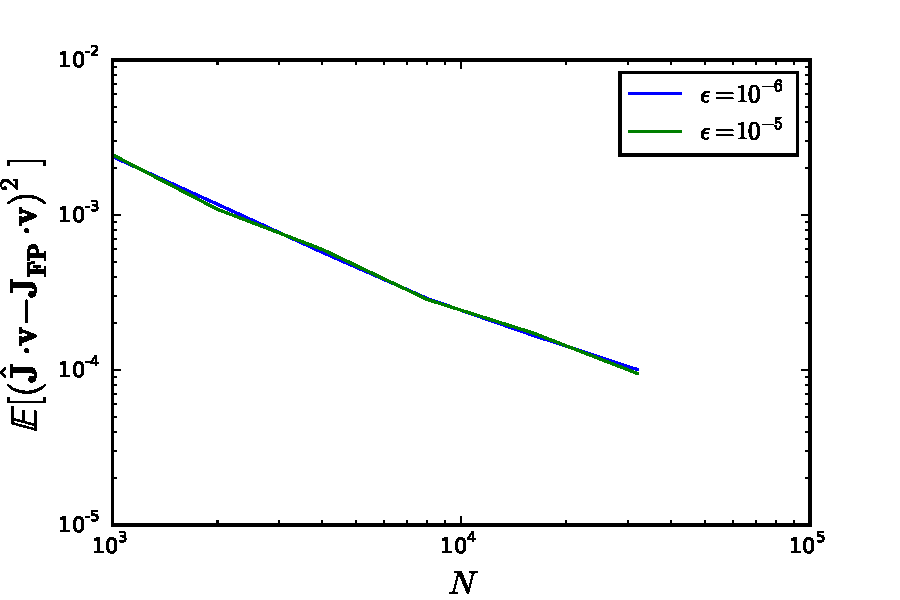
\includegraphics{../results/plots/ms_Jveps-5eps-6}
%\caption{}
%\label{Convergence_Jv}
%\end{figure}



%\subsection{Results}
%
%From now on, let us abbreviate the Jacobian-vector product $D(\cts) \cdot \mathbf{v}$  estimated from the for particle-based time-stepper as $\jv$.  We also chose the perturbation vector $\V$ to be sinusiodal  (the convergence plots will be  independent from $\V$). If we calculate $\jv$ from the stochastic simulations with different number of particles $N$, we can test two things: the convergence to zero of the variance on $\jv$ and the convergence to zero of the estimated bias on $\jv$.  We will also plot the mean squared error (MSE) which incorporates both effects (see eq. \eqref{MSE}. 
%The bias can be estimated by comparing the expectation value $\norm{\jv}$ with the Jacobian-vector product for the PDE solved on a fine grid, denoted as $\jvpde$. The estimated expectation value $\mathbb{E}(\jv)$ is the Jacobian-vector averaged over $M$ stochastic simulations. 
%
%%\begin{equation} \label{MSE}
%%\texttt{MSE}(\jv, \mathbf{\bar{Jv} }) = \frac{ \mathbb{E} \left[   \left(  \jv - \mathbf{\bar{Jv}}  \right)^T  \cdot  \left(  \jv - \mathbf{\bar{Jv}}  \right) \right]} {n_x}  =    \texttt{Var}(\jv) +  \left( \texttt{Bias} (\jv)\right)^T \cdot  \left( \texttt{Bias} (\jv)\right)
%%\end{equation}
%%with 
%%\begin{equation} \nonumber
%% \texttt{Var}(\hat{Jv}) = \frac{ \mathbb{E} \left[   \left(  \jv - \mathbb{E}[\jv]   \right)^T  \cdot  \left(   \jv - \mathbb{E}[\jv]    \right) \right]} {n_x} 
%%\end{equation}
%
%
%\begin{equation} \label{MSE}
%\texttt{MSE}(\jv, \jvpde ) =  \mathbb{E} \left[   \left(  \jv - \jvpde  \right)^2 \right]  =   \texttt{Var}(\jv) +  \left( \mathbf{Bias}(\jv, \jvpde )  \right)^2
%\end{equation}
%with 
%\begin{equation} \label{Var}
% \texttt{Var}(\jv) =  \mathbb{E} \left[   \left(  \jv - \mathbb{E}[\jv]   \right)^2 \right] 
%\end{equation}
%and 
%\begin{equation} 
% \mathbf{Bias}(\jv, \jvpde ) = \mathbb{E}[\jv]  - \jvpde ,
%\end{equation}
%where we defined the inproduct of a $n_x$-dimensional vector $\V$ as $\mathbf{v}^2 = \frac{\V^T \cdot \V}{n_x}$. Thus, in eq. \eqref{MSE} and \eqref{Var} we divide by the number of discretization steps $n_x$ \footnote{If the number of discretisations steps for solving the PDE happens to be  higher than the number of bins $n_x$, we rescale the dimension of $\jvpde$ to $n_x$}. This allows us to make a meaningful comparison with solutions on finer or coarser grids. 
%
%
%
%%\begin{figure}
%%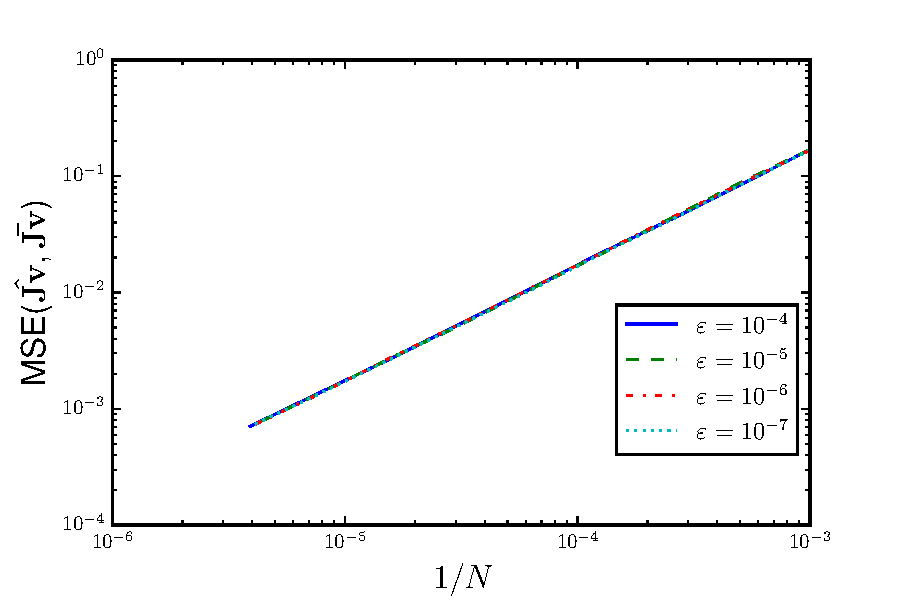
\includegraphics[width=14.5cm]{../Problems/WeightedParticles/checkSystem/plots/MSE_N_eps}
%%\caption{The mean squared error between the stochastic and the deterministic solution for the Jacobian-vector-product converges to zero with $\mathcal{O}(1/ N)$ and it does not depend on the value of $\varepsilon$.}
%%\label{MSE_N}
%%\end{figure}
%%
%\begin{figure}
%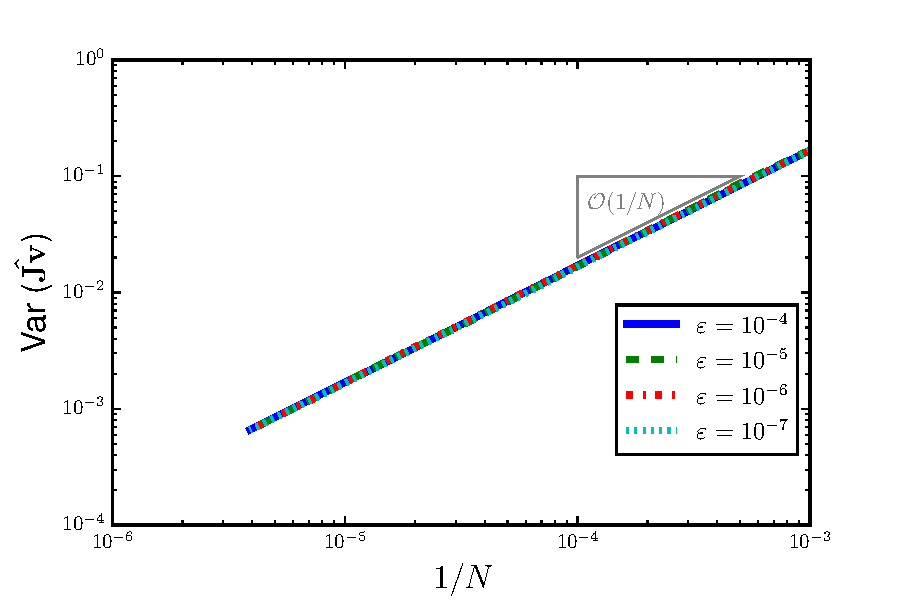
\includegraphics[width=14.5cm]{../Problems/WeightedParticles/checkSystem/plots/Var_N_eps}
%\caption{The variance on the stochastic solution for the Jacobian-vector-product converges to zero with $\mathcal{O}(1/ N)$ and it does not depend on the value of $\varepsilon$.}
%\label{Var_N}
%\end{figure}



%\begin{figure}
%\centering
%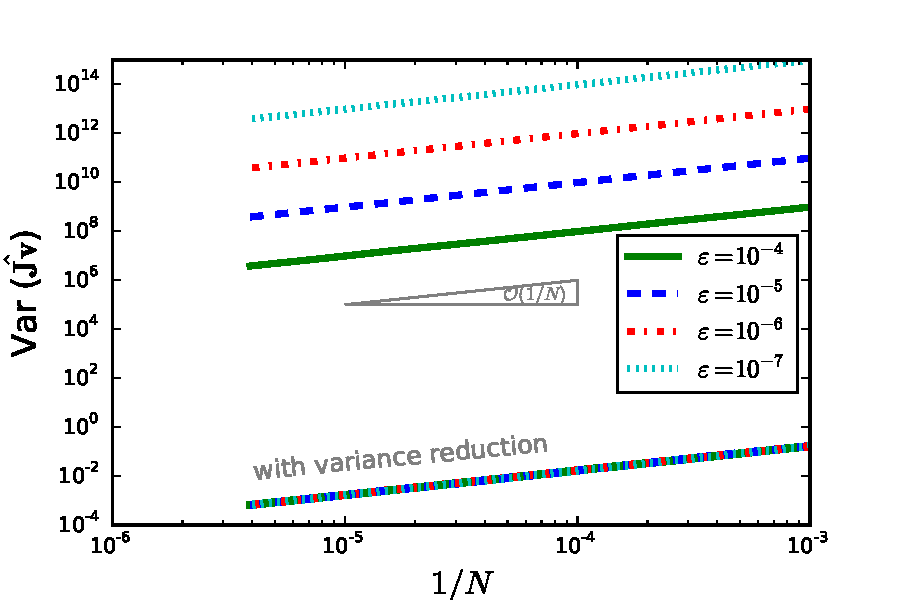
\includegraphics[width=0.8\linewidth]{../Problems/Particles/checkSystem/plots/Var_N_eps_nw}
%\caption[Effect of variance reduction]{In the case of unweighted restriction, the variance on the stochastic solution of the Jacobian-vector-product becomes unbounded as we decrease the perturbation size $\epsilon$. By using weights in the restriction step, the variance does not longer depend on the value of $\varepsilon$ and   converges to zero with $\mathcal{O}(1/ N)$.}
%\label{Var_N}
%\end{figure}


%
%%\begin{figure}
%%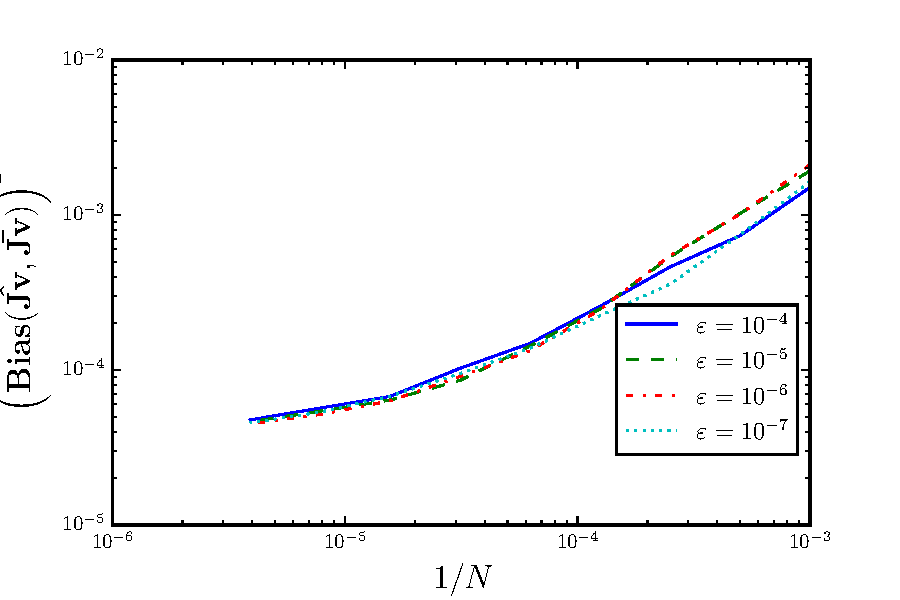
\includegraphics[width=14.5cm]{../Problems/WeightedParticles/checkSystem/plots/Bias_N_eps}
%%\caption{The squared bias between the stochastic and the deterministic solution for the Jacobian-vector-product does not depend on the value of $\varepsilon$.}
%%\label{Bias_N}
%%\end{figure}
%
%
%
%%
%%\begin{figure}
%%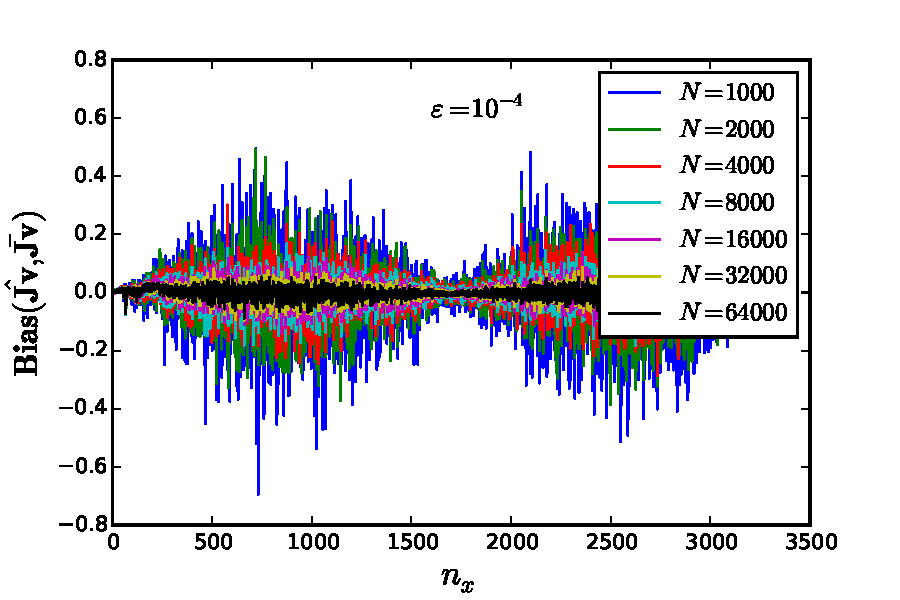
\includegraphics[width=8.5cm]{../Problems/WeightedParticles/checkSystem/plots/25-11Bias_e-_4}
%%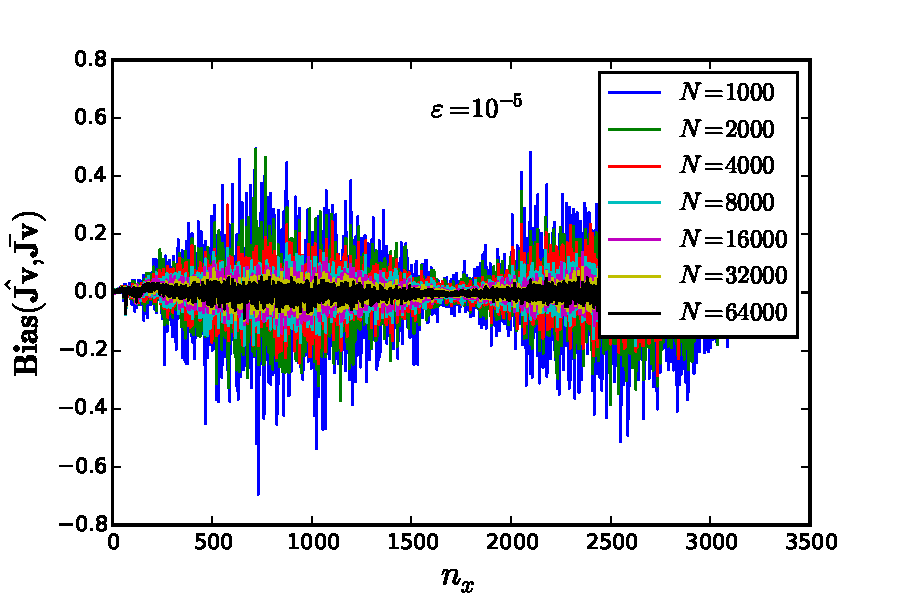
\includegraphics[width=8.5cm]{../Problems/WeightedParticles/checkSystem/plots/25-11Bias_e-_5}
%%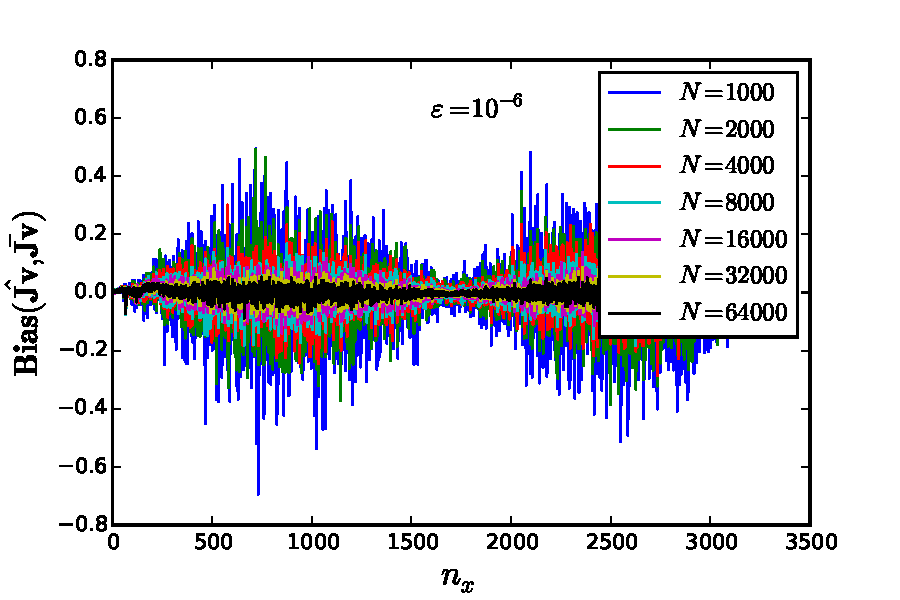
\includegraphics[width=8.5cm]{../Problems/WeightedParticles/checkSystem/plots/25-11Bias_e-_6}
%%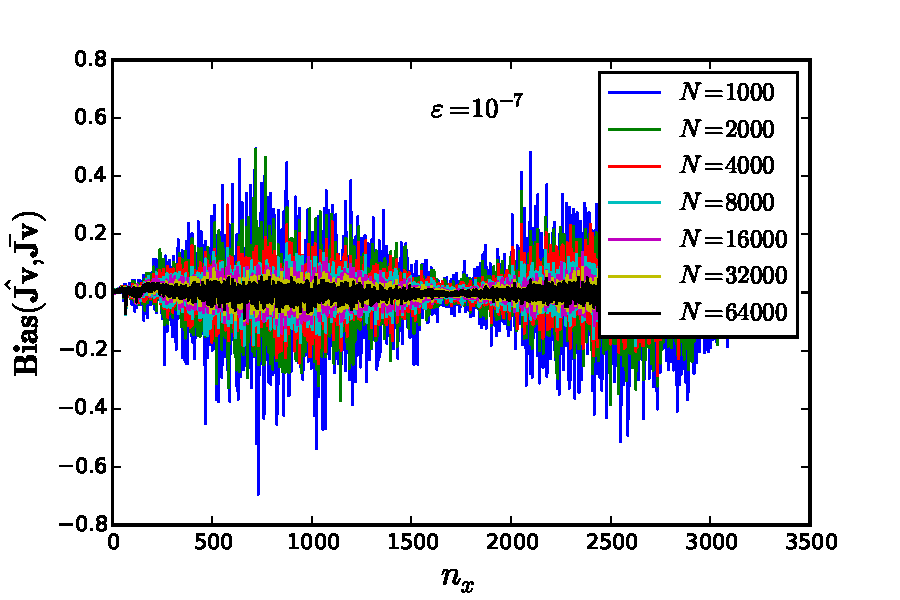
\includegraphics[width=8.5cm]{../Problems/WeightedParticles/checkSystem/plots/25-11Bias_e-_7}
%%\caption{The bias on the stochastic solution for the Jacobian-vector-product converges to zero if the number of particles is increased and it does not depend on the value of $\varepsilon$.}
%%\label{bias_v}
%%\end{figure}
%%
%
%
%
%
%
%\begin{table}
%
%\caption{Parameter values}
%   %FTCS-scheme  &   Euler-Maruyama-scheme  \\
% 
%     \begin{tabular} { | c  c | c | c |}    \hline   
%     %FTCS-scheme  &   Euler-Maruyama-scheme  \\  
%   \textit{ {Discretization parameters}}    &  & PDE  & SDE  \\ \hline
%    Discretization step  & $\Delta x $ & $10^{-4}$  & $10^{-2}$ \\ 
%        Number of discretization steps &  $n_x$ &  $34 000$ & 340 \\ 
%    Time step  &  $\Delta t$ & $10^{-8}$ &  $10^{-4}$ \\ 
%       Number of timesteps  & $n$  &  $10^{6}$ &  100   \\ \hline
%  \end{tabular}
%\quad
%     \begin{tabular}  { | c | c | c |  }  \hline
%     \multicolumn{3}{|c|} {\textit{ System parameters}   }    \\
%    \hline  
%    Diffusion coefficient  & $D $ & $0.5$ \\ 
%   Drift coefficient &  $a$ & $ 1$ \\ \hline
%  \multicolumn{3}{|c|} {\textit{ Simulation parameters}   }    \\ \hline
%   Number of realizations  & $M $ & $100$ \\ \hline
%    Perturbation size & $\varepsilon$  & $ 10^{-5}$ \\ \hline
%  \end{tabular}
%
%\end{table}
%
%
%
%
%%Total simulation time for particle-based time-stepper 
%%
%%Total Simulation time for PDE-based time stepper
%
%%\subsection{Variance}
%%\begin{equation}
%%\mathbb{E} \left[ (\rho -\mathbb{E}[\rho ])^2 \right] =?
%%\end{equation}
%%
%%
%%
%
%%\begin{equation}
%%D(\cts) \cdot \mathbf{v} \approx  \frac{\cts (\U, \boldsymbol{\omega_1} )  + \varepsilon \mathbf{v}  - \cts (\U, \boldsymbol{\omega_2}) }{\varepsilon} 
%%\end{equation}
%
%
%
%
%%\subsection{Convergence}
%
%%\section{Some documentation about the use of random numbers in the simulation}
%%
%%Every MC-step starts with a new seed for seeding the density sampler in the lifting step. This same seed is used for the time evolution of every particle. So, for a given MC-step and a given timestep, the brownian increment is the same for all particles in the simulation. This means that the sum of all Brownian steps is the same for all particles. This does not mean that $\Delta(x+\Delta T) - \Delta(x)$ is the same for all particles, because this depends on the drift-term, which depends on the position, which is different for every particle.
%
%
%\section{Convergence of the bias}
%We calculate the expectation value of $\jv$ by substituting eq. \eqref{} in the finite-difference approximation.
%
%\begin{equation}
%\E[\jv] =  \E \left[ \frac{\cts (\hat{\U} + \varepsilon \mathbf{v} )  - \cts (\hat{\U})}{\varepsilon}  \right]
%\end{equation}
%with \begin{equation}
%\cts (\hat{\U})  = \frac{1}{N}\sum_{i=1}^{N} \chi_{\Delta_j} \left[\mathcal{E} (x_i(t) \right]
%\end{equation}
%and 
%\begin{equation}
%\cts (\hat{\U} + \varepsilon \V )  = \frac{1}{N}\sum_{i=1}^{N}  (1+ \frac{\varepsilon \V}  {\U(x_i(t))}  ) \cdot \chi_{\Delta_j} \left[\mathcal{E} (x_i(t) \right] .
%\end{equation}
%
%
%\begin{eqnarray}
%\E[\jv] &=&  \E \left[  \frac{1}{N}\sum_{i=1}^{N}   \frac{ \chi_{\Delta_j} \left[  \mathcal{E} (x_i(t)) \right] \V}  {\U(x_i(t))}     \right] \\
%		&=&   \frac{\V}{N} \E \left[  \sum_{i=1}^{N}   \frac{ \chi_{\Delta_j} \left[  \mathcal{E} (x_i(t)) \right] }  {\U(x_i(t))}     \right] \\
%		&=&  \frac{\V}{N}  \sum_{i=1}^{N}   \frac{  \E \left[  \chi_{\Delta_j} \left[  \mathcal{E} (x_i(t)) \right]  \right] }  {\U(x_i(t))} \\
%		&=& \frac{\V}{N}  \sum_{i=1}^{N}   \frac{  \chi_{\Delta_j} \left[  \E \left[   \mathcal{E} (x_i(t)) \right]  \right] }  {\U(x_i(t))} 
%\end{eqnarray}
%
%
%
%%\begin{eqnarray}
%%\E[\jv] &=&  \E \left[ \frac{\cts (\hat{\U} + \varepsilon \mathbf{v} )  - \cts (\hat{\U})}{\varepsilon}  \right]
%%        &=&  \E \left[ \frac{1}{N} ] 
%%\end{eqnarray}
%
%\begin{figure}
%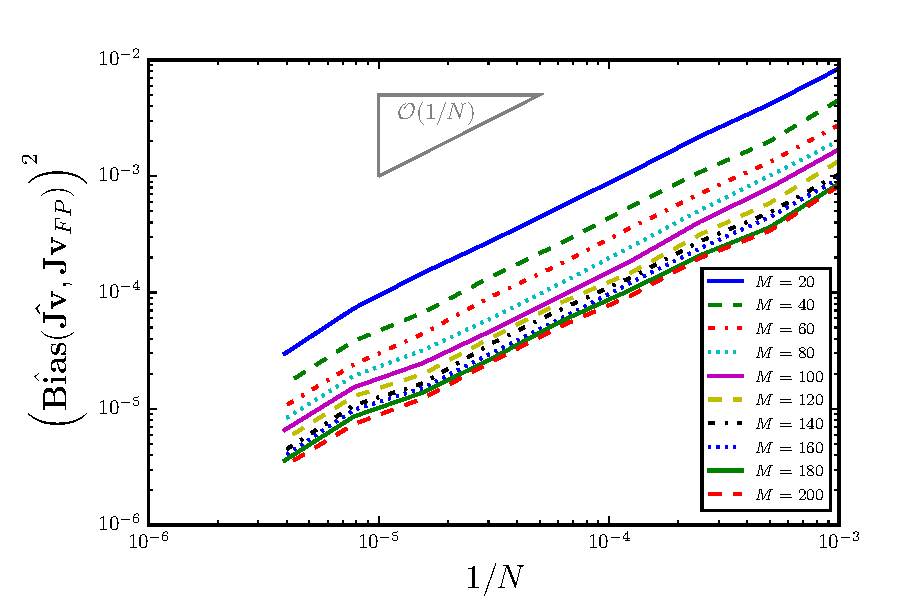
\includegraphics[width=14.5cm]{../Problems/WeightedParticles/checkSystem/plots/Bias_Jv_N_M.pdf}
%\caption{The expectation value of the stochastic solution of the Jacobian-vector-product is calculated by averaging over $M$ stochastic realizations. The estimated bias between this solution and the deterministic one is squared and plotted as a function of the number of particles $N$ for different values of $M$.  For large particle numbers, the estimated bias becomes independent of $M$ and converges to the real bias. This real bias is the numerical error in the solution of the PDE [Need to check this last statement].}
%\label{Bias_Jv_N_M}
%\end{figure}
%
%
%\begin{figure}
%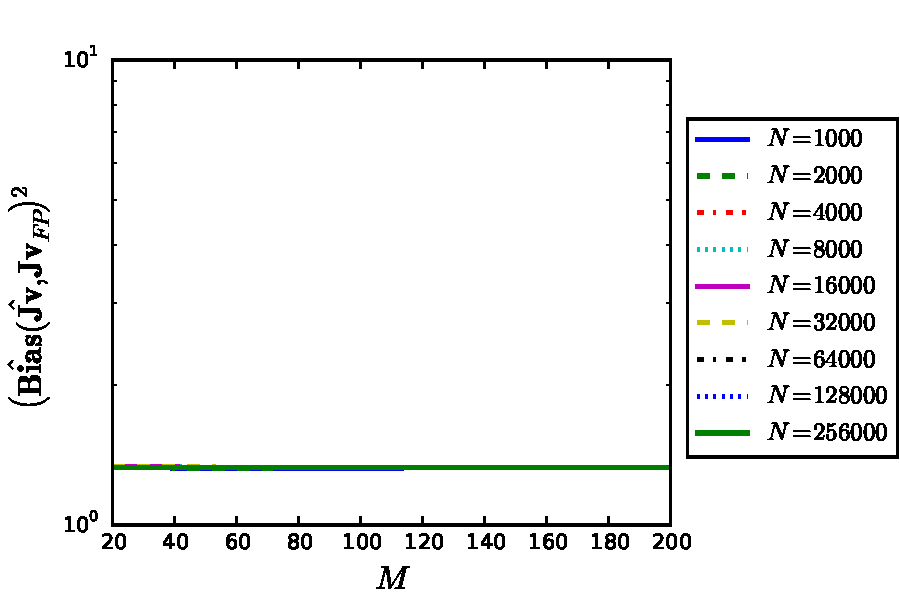
\includegraphics[width=14.5cm]{../Problems/WeightedParticles/checkSystem/plots/Bias_Jv_M_N.pdf}
%\caption{The expectation value of the stochastic solution of the Jacobian-vector-product is calculated by averaging over $M$ stochastic realizations. The estimated bias between this solution and the deterministic one is squared and plotted as a function of the number of realizations $M$ for simulations with different particle number $N$.  For large particle numbers, the estimated bias becomes independent of $M$ and converges to the real bias. This real bias is the numerical error in the solution of the PDE [Need to check this last statement].}
%\label{Bias_Jv_M_N}
%\end{figure}-
%
%\begin{itemize}
%\item
%\end{itemize}
%
%
%%\section{Simulation}
%%\subsection{Default input values}
%%
%%
%%\begin{itemize}
%%\item $\varepsilon  =10^{-5}$
%% \item $ N =10 000$
%%\end{itemize}
%





\section{Method}
\subsection{Coarse time stepper}


To simulate the time evolution of  the density $\U(t)$, we construct  a coarse time stepper $\cts$ which allows the performance of time-steps at the macroscopic level, using only the stochastic simulation of the position vectors of the $N$ particles at the microscopic level, %$\mathbf{X}(t+ n \Delta t)$, 
generated by eq. \eqref{Euler-Mar}. 

To achieve this, we will define two operators (lifting in subsection \ref{section:lifting} and
restriction in subsection \ref{section:restriction}) that relate the microscopic and macroscopic levels of description.
Once these lifting $\mathcal{L}$ and restriction  operators $\mathcal{R}$ have been constructed, a coarse time-stepper $\cts$ 
to evolve the macroscopic state $\U$ over a time interval of length $n \Delta t$ is constructed as a three-step-procedure (lift–evolve–restrict):

\begin{equation}
\U(t + n \Delta t) = \cts(\U) = (\mathcal{R} \circ \mathcal{E}(n \Delta t) \circ  \mathcal{L}(\mathbf{\omega})  ) (\U(t))
\end{equation}
where $\mathcal{E}(n \Delta t)(\U(t))$ is the simulation of the SDE for $N$ particles over $n$ timesteps.


\subsubsection{Lifting: $\U \rightarrow \mathbf{X} $} \label{section:lifting}
Given the density \U, we need to sample a position vector $X_i$ for every particle $i \leq N$. We compute $X$ from a $N$-dimensional vector $\bf{U}$  with uniform random elements $U_i \in [0,1]$ such that $\U(X_i)=U_i$, using the inverse transformation method. The particle does not only gets an inital position, but also a seed for generating random steps in the simulation.

\subsubsection{Restriction:  $\mathbf{X} \rightarrow \U $}
\label{section:restriction}
The restriction operator $\mathcal{R}: \mathbb{Q}^N \rightarrow \mathbb{Q}^k$ maps the microscopic state $\mathbf{X}$ (determined by the position vectors of $N$ particles) to a density \U, discretisized in $k$ bins. This is done by counting the number of particles in every bin $\Delta_j$ for $1\leq j \leq k$: %= x_{j+\frac{1}{2}}-x_{j-\frac{1}{2}}$. 

\begin{equation}
\frac{1}{N} \sum_{i=1}^{N}  w^i \cdot \chi_{\Delta_j}(X^i) = \rho_j  \label{restriction}
\end{equation}
with 
\begin{equation}
\chi_{\Delta_j}(X) = \begin{cases}
  1 & \mbox{if } X \in \Delta_j, \\
  0 & \mbox{if } X \notin \Delta_j. \\
\end{cases}
\end{equation}
%\begin{equation}
% \frac{1}{k}\sum_{j=1}^{k} \rho_j =  \frac{1}{N} \sum_{i=1}^{N}  w_i x_i
%\end{equation}
and setting all weights $w_i =1 $ for $1\leq i \leq N$.

The reason why we explicitly introduced these weights in the restriction operator will be clarified in section \ref{Jv_approx} where we will need to evaluate  the coarse time stepper  $\cts (\U + \varepsilon \mathbf{v})$, now applied to the density shifted with a certain perturbation $\varepsilon \mathbf{v}$. %We explicitly introduced these weights in the restriction operator \eqref{restriction} because they can help to reduce the variance in the jacobian-vector-products. In the finite difference approximation we need to evaluate $\cts (\U + \varepsilon \mathbf{v})$, the coarse time stepper applied to the density shifted with a certain perturbation.
%For the weighted restriction operator, we choose different weights $w_i$ for every particle. (we only use this for calculating the jacobian-vector-produ cts. (Why? Well, the weights are just one if we dont use a perturbation)f
To evaluate the perturbated restriction-operator we will use the weights $ w^i_{\varepsilon}$, determined such that
\begin{equation}
\frac{1}{N} \sum_{i=1}^{N}  w^i_{\varepsilon} \cdot \chi_{\Delta_j} (X^i) = \rho_j + \varepsilon v_j . \label{restriction_eps}
\end{equation}
We do this by computing the weight per bin as $ w^j_{\varepsilon} = 1+ \frac{\varepsilon v_j}{\rho_j}$ and assign this value to each particle in $\Delta_j$. So, small perturbations on the density lead to small perturbations in the weights. The advantage of this weighted restriction operator lies in the possibility to use the same realizations $\mathbf{X}$ in the unperturbated \eqref{restriction} and the perturbated  \eqref{restriction_eps} restriction-operator.



%
%\bibliographystyle{plain}
%\bibliography{biblio.bib}





\end{document}
